\chapter{Les molécules organiques~: squelettes et noms}\label{ch:g11:organic-skeletons}

Un briquet jetable contient du butane, liquide sous pression~; la
cartouche d'un réchaud emporté sur une montagne enneigée contient du
propane, ou un \omterm{def:g6:pure-substances-and-mixtures:mixture}{mélange} qui en est plus riche. Tous deux ne sont faits
que d'\omterm{def:g7:atoms-and-molecules:atom}{atomes} de carbone et d'hydrogène, et tous deux appartiennent à une
immense famille~: celle des \omterm{def:g7:atoms-and-molecules:molecule}{molécules} construites sur un squelette
d'\omterm{def:g7:atoms-and-molecules:atom}{atomes} de carbone. On en connaît des millions. Pour en parler, les
chimistes ont besoin de moyens de les dessiner rapidement et de les
nommer sans ambiguïté.

\begin{recall}
Le carbone forme quatre \omterm{def:g10:lewis-and-shape:covalent-bond}{liaisons covalentes} et l'hydrogène une seule~;
autour d'un \omterm{def:g7:atoms-and-molecules:atom}{atome} de carbone engagé dans quatre liaisons simples, les
liaisons pointent vers les sommets d'un tétraèdre, à environ
\ang{109.5} (\cref{ch:g10:lewis-and-shape}).
\end{recall}

\begin{omfigure}
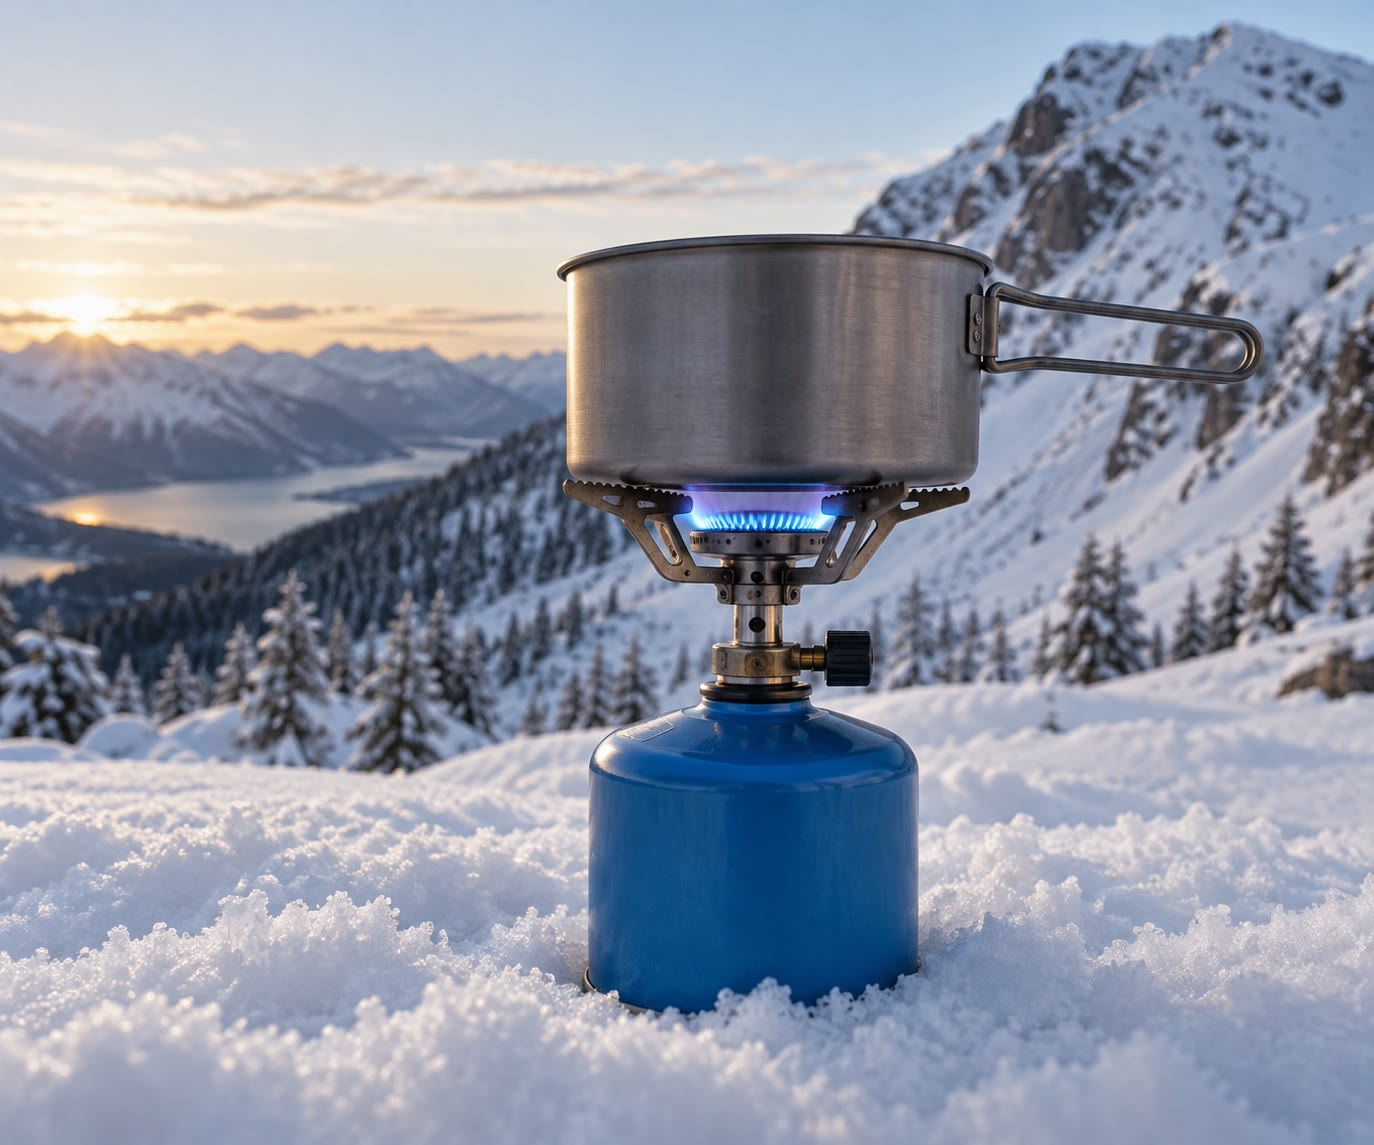
\includegraphics[width=0.48\linewidth]{images/book1/ai/g11-camping-cartridge.jpg}

{\small Un réchaud de camping dans la neige, qui \omterm{def:g4:what-a-fire-needs:burning}{brûle} un gaz fait de
carbone et d'hydrogène.}
\end{omfigure}

\section{Les formules des molécules organiques}

\begin{definition}[Composé organique]\label{def:g11:organic-skeletons:organic}
Un \emph{composé organique}\index{compose organique@composé organique} est un composé dont
les \omterm{def:g7:atoms-and-molecules:molecule}{molécules} sont construites sur un squelette d'\omterm{def:g7:atoms-and-molecules:atom}{atomes} de carbone liés
entre eux et à des \omterm{def:g7:atoms-and-molecules:atom}{atomes} d'hydrogène, avec éventuellement d'autres
\omterm{def:g7:atoms-and-molecules:atom}{atomes} comme l'oxygène et l'azote. (Le dioxyde de carbone, le monoxyde
de carbone et les carbonates en sont traditionnellement exclus.)
\end{definition}

\begin{definition}[Quatre sortes de formules]\label{def:g11:organic-skeletons:formulas}
Une \omterm{def:g7:atoms-and-molecules:molecule}{molécule} peut s'écrire de quatre façons~:
\begin{itemize}
  \item sa \emph{formule brute}\index{formule brute} donne seulement le
        nombre d'\omterm{def:g7:atoms-and-molecules:atom}{atomes} de chaque élément, comme \ce{C4H10}~;
  \item sa \emph{formule développée}\index{formule developpee@formule développée} montre
        tous les \omterm{def:g7:atoms-and-molecules:atom}{atomes} et toutes les liaisons~;
  \item sa \emph{formule semi-développée}\index{formule semi-developpee@formule semi-développée}
        montre les liaisons entre \omterm{def:g7:atoms-and-molecules:atom}{atomes} de carbone et regroupe les \omterm{def:g7:atoms-and-molecules:atom}{atomes}
        d'hydrogène avec leur carbone, comme \ce{CH3-CH2-CH2-CH3}~;
  \item sa \emph{formule topologique}\index{formule topologique} ne
        dessine que les liaisons du squelette carboné, en zigzag~: chaque
        extrémité et chaque sommet est un \omterm{def:g7:atoms-and-molecules:atom}{atome} de carbone, les \omterm{def:g7:atoms-and-molecules:atom}{atomes}
        d'hydrogène portés par le carbone ne sont pas dessinés, et tout
        autre \omterm{def:g7:atoms-and-molecules:atom}{atome} (avec ses \omterm{def:g7:atoms-and-molecules:atom}{atomes} d'hydrogène) est écrit.
\end{itemize}
\end{definition}

\begin{omfigure}
\setchemfig{atom sep=1.45em}
\renewcommand{\arraystretch}{1.6}
\small
\begin{tabular}{@{}l@{\quad}c@{\quad}c@{}}
 & butane & 2-méthylpropane \\
brute & \ce{C4H10} & \ce{C4H10} \\[4pt]
développée &
\chemfig{H-C(-[2]H)(-[6]H)-C(-[2]H)(-[6]H)-C(-[2]H)(-[6]H)-C(-[2]H)(-[6]H)-H} &
\chemfig{H-C(-[2]H)(-[6]H)-C(-[6]H)(-[2,1.5]C(-[1]H)(-[3]H)(-[2]H))-C(-[2]H)(-[6]H)-H} \\[10pt]
semi-développée & \ce{CH3-CH2-CH2-CH3} &
\chemfig{CH_3-CH(-[6]CH_3)-CH_3} \\[14pt]
topologique & \chemfig{-[:30]-[:-30]-[:30]} & \chemfig{-[:30](-[:90])-[:-30]} \\
\end{tabular}

{\small Les quatre formules du butane et du 2-méthylpropane. Dans les
\omterm{def:g11:organic-skeletons:formulas}{formules topologiques}, chaque extrémité et chaque sommet des traits est
un \omterm{def:g7:atoms-and-molecules:atom}{atome} de carbone~: quatre dans chacune.}
\end{omfigure}


\begin{example}[Lire une formule topologique]\label{ex:g11:organic-skeletons:reading}
Dans la \omterm{def:g11:organic-skeletons:formulas}{formule topologique} du butane, le zigzag a deux extrémités et
deux sommets~: quatre \omterm{def:g7:atoms-and-molecules:atom}{atomes} de carbone. Chaque carbone d'extrémité n'a
qu'une liaison dessinée~: il porte donc trois \omterm{def:g7:atoms-and-molecules:atom}{atomes} d'hydrogène
(\ce{CH3})~; chaque sommet a deux liaisons dessinées~: il en porte deux
(\ce{CH2}). Chaque carbone a quatre liaisons en tout, ce qui redonne
\ce{C4H10}.
\end{example}

\section{Les chaînes carbonées}

Le squelette carboné d'une \omterm{def:g7:atoms-and-molecules:molecule}{molécule} peut être une chaîne
\emph{linéaire}, chaque carbone étant lié à deux autres au plus, comme
dans le butane~; une chaîne \emph{ramifiée}, avec au moins un carbone lié
à trois ou quatre autres, comme dans le 2-méthylpropane~; ou un
\emph{cycle}, comme dans le cyclohexane, \ce{C6H12}, dont la \omterm{def:g11:organic-skeletons:formulas}{formule
topologique} est un hexagone. On dessine les chaînes en zigzag parce que
les liaisons réelles autour de chaque carbone forment des angles
d'environ \ang{109.5}, et non de \ang{180}~: une chaîne «~linéaire~»
est en fait un zigzag dans l'espace.

\begin{omfigure}
\setchemfig{atom sep=1.9em}
\begin{tabular}{ccc}
\chemfig{-[:30]-[:-30]-[:30]-[:-30]-[:30]} &
\chemfig{-[:30](-[:90])-[:-30]-[:30](-[:90])-[:-30]} &
\chemfig{*6(------)} \\[4pt]
\small linéaire~: hexane & \small ramifiée~: 2,4-diméthylpentane &
\small cyclique~: cyclohexane \\
\small \ce{C6H14} & \small \ce{C7H16} & \small \ce{C6H12}
\end{tabular}

{\small Trois squelettes carbonés, en \omterm{def:g11:organic-skeletons:formulas}{formules topologiques}.}
\end{omfigure}

\section{Les alcanes et leurs noms}

\begin{definition}[Alcane, groupe alkyle]\label{def:g11:organic-skeletons:alkane}
Un \emph{alcane}\index{alcane} est un composé de carbone et d'hydrogène
dont le squelette est une chaîne (linéaire ou ramifiée, pas un cycle) ne
comportant que des liaisons simples~; sa \omterm{def:g11:organic-skeletons:formulas}{formule brute} est
\ce{C_{n}H_{2n+2}}. Un \emph{groupe
alkyle}\index{groupe alkyle} est ce qui reste d'un alcane quand on lui
retire un \omterm{def:g7:atoms-and-molecules:atom}{atome} d'hydrogène, pour pouvoir le fixer à une chaîne~:
méthyle \ce{-CH3}, éthyle \ce{-CH2-CH3}.
\end{definition}

\begin{omfigure}
\begin{tabular}{rlcrlc}
\hline
$n$ & nom & formule & $n$ & nom & formule \\
\hline
1 & méthane & \ce{CH4}    & 6  & hexane & \ce{C6H14} \\
2 & éthane  & \ce{C2H6}   & 7  & heptane & \ce{C7H16} \\
3 & propane & \ce{C3H8}   & 8  & octane & \ce{C8H18} \\
4 & butane  & \ce{C4H10}  & 9  & nonane & \ce{C9H20} \\
5 & pentane & \ce{C5H12}  & 10 & décane & \ce{C10H22} \\
\hline
\end{tabular}\par\medskip

{\small Les dix premiers \omterm{def:g11:organic-skeletons:alkane}{alcanes} linéaires. Le nom d'une chaîne de $n$
\omterm{def:g7:atoms-and-molecules:atom}{atomes} de carbone est formé d'un même radical suivi de \emph{-ane}~; le
\omterm{def:g11:organic-skeletons:alkane}{groupe alkyle} remplace \emph{-ane} par \emph{-yle} (méthyle, éthyle,
propyle\dots).}
\end{omfigure}

\begin{method}[Nommer un alcane]\label{met:g11:organic-skeletons:naming}
\begin{enumerate}
  \item Trouver la plus longue chaîne d'\omterm{def:g7:atoms-and-molecules:atom}{atomes} de carbone~: elle donne le
        nom de base (pentane, hexane\dots).
  \item Les \omterm{def:g7:atoms-and-molecules:atom}{atomes} qui n'en font pas partie forment des \omterm{def:g11:organic-skeletons:alkane}{groupes alkyle}
        fixés sur elle, les substituants.
  \item Numéroter la chaîne principale à partir de l'extrémité qui donne
        aux substituants les numéros les plus petits.
  \item Écrire chaque substituant avec son numéro (sa position sur la
        chaîne), par ordre alphabétique, devant le nom de base~; les
        groupes répétés prennent les préfixes di-, tri-, tétra-, avec un
        numéro pour chacun. Les numéros sont séparés par des virgules, les
        numéros et les mots par des tirets.
\end{enumerate}
\end{method}

\begin{omfigure}
\begin{tikzpicture}[font=\small, x=0.9cm, y=0.9cm]
  % main chain of 5, zigzag; methyls on C2 and C3
  \coordinate (a1) at (0,0); \coordinate (a2) at (0.87,0.5);
  \coordinate (a3) at (1.73,0); \coordinate (a4) at (2.6,0.5);
  \coordinate (a5) at (3.46,0);
  \coordinate (m2) at (0.87,1.5); \coordinate (m3) at (1.73,-1);
  \draw[line width=1pt] (a1) -- (a2) -- (a3) -- (a4) -- (a5);
  \draw[line width=1pt] (a2) -- (m2); \draw[line width=1pt] (a3) -- (m3);
  \foreach \k in {1,2,3,4,5}
    \node[omDef, font=\footnotesize\bfseries, fill=white, inner sep=1pt]
      at ($(a\k)+(0,-0.32)$) {\k};
  \draw[omProp, thick] (m2) circle (0.28);
  \draw[omProp, thick] (m3) circle (0.28);
  \node[omProp, anchor=west] at ($(m2)+(0.35,0)$) {méthyl sur C2};
  \node[omProp, anchor=west] at ($(m3)+(0.35,0)$) {méthyl sur C3};
  \node[anchor=west, align=left] at (5,0.3) {plus longue chaîne~: 5 carbones,
    \emph{pentane}\\ numérotée par la gauche~: 2 et 3\\ (par la droite~: 3
    et 4, plus grands)\\ nom~: \textbf{2,3-diméthylpentane}};
\end{tikzpicture}

{\small Nommer un \omterm{def:g11:organic-skeletons:alkane}{alcane} ramifié~: la chaîne principale (numérotée), les
substituants (entourés), le nom.}
\end{omfigure}

\begin{method}[D'un nom à une formule topologique]\label{met:g11:organic-skeletons:drawing}
\begin{enumerate}
  \item Dessiner en zigzag la chaîne principale donnée par le nom de
        base, et numéroter ses carbones.
  \item Fixer chaque substituant à la position donnée par son numéro.
  \item Vérifier~: compter les carbones, et s'assurer qu'aucun carbone
        n'a plus de quatre liaisons.
\end{enumerate}
\end{method}

\section{Les isomères}

\begin{definition}[Isomères, isomères de constitution]\label{def:g11:organic-skeletons:isomer}
Des \emph{isomères}\index{isomere@isomère} sont des composés différents qui ont
la même \omterm{def:g11:organic-skeletons:formulas}{formule brute}. Des
\emph{isomères de constitution}\index{isomere de constitution@isomère de constitution} sont des
isomères dont les \omterm{def:g7:atoms-and-molecules:atom}{atomes} sont liés dans un ordre différent, par exemple
avec un squelette carboné différent.
\end{definition}

\begin{proposition}[Les isomères ont des propriétés différentes]\label{prop:g11:organic-skeletons:properties}
% ledger: bp:C4H10, bp:isobutane, bp:C5H12, bp:isopentane, bp:neopentane
Des \omterm{def:g11:organic-skeletons:isomer}{isomères de constitution} sont des substances différentes, aux
propriétés différentes. Parmi les \omterm{def:g11:organic-skeletons:alkane}{alcanes} \omterm{def:g11:organic-skeletons:isomer}{isomères} d'une même formule,
les plus ramifiés bouillent le plus bas~: le butane bout vers
\qty{0}{\celsius} et le 2-méthylpropane à \qty{-11.7}{\celsius}~; le
pentane à \qty{36.1}{\celsius}, le 2-méthylbutane à \qty{27.8}{\celsius}
et le 2,2-diméthylpropane à \qty{9.5}{\celsius}.
\end{proposition}

\begin{proof}
Les valeurs sont des mesures. Les \omterm{def:g7:atoms-and-molecules:molecule}{molécules}
ramifiées sont plus compactes, avec moins de surface en contact avec
leurs voisines~: leurs \omterm{def:g11:polarity-and-cohesion:van-der-waals}{interactions de van der Waals} sont plus faibles
(\cref{ch:g11:polarity-and-cohesion}).
\end{proof}

\begin{omfigure}
\setchemfig{atom sep=2em}
\begin{tabular}{ccc}
\chemfig{-[:30]-[:-30]-[:30]-[:-30]} &
\chemfig{-[:30](-[:90])-[:-30]-[:30]} &
\chemfig{-[:0](-[:90])(-[:-90])-[:0]} \\[24pt]
\small pentane & \small 2-méthylbutane & \small 2,2-diméthylpropane \\
\small \qty{36.1}{\celsius} & \small \qty{27.8}{\celsius} &
\small \qty{9.5}{\celsius}
\end{tabular}
\medskip

{\small Les trois \omterm{def:g11:organic-skeletons:isomer}{isomères} de \ce{C5H12} et leurs températures
d'ébullition~: plus la \omterm{def:g7:atoms-and-molecules:molecule}{molécule} est ramifiée, plus elle est basse.}
\end{omfigure}

\section{Les alcanes du pétrole}

Le pétrole brut est un \omterm{def:g6:pure-substances-and-mixtures:mixture}{mélange} de milliers de composés, pour la plupart
des \omterm{def:g11:organic-skeletons:alkane}{alcanes} de 1 à plus de 40 \omterm{def:g7:atoms-and-molecules:atom}{atomes} de carbone. Dans une raffinerie, on
le chauffe et ses vapeurs montent dans une haute colonne, de plus en
plus froide vers le haut~: chaque fraction se condense à la hauteur où
la température correspond à son domaine d'ébullition. Les gaz (du
méthane au butane) sortent en haut, puis l'essence, le kérosène, le
gazole~; les huiles lourdes et le bitume restent en bas. Cette
\omterm{def:g10:chemical-species:distillation}{distillation} fractionnée sépare selon la température d'ébullition, qui,
pour les \omterm{def:g11:organic-skeletons:alkane}{alcanes}, augmente avec la longueur de la chaîne.

\begin{omfigure}
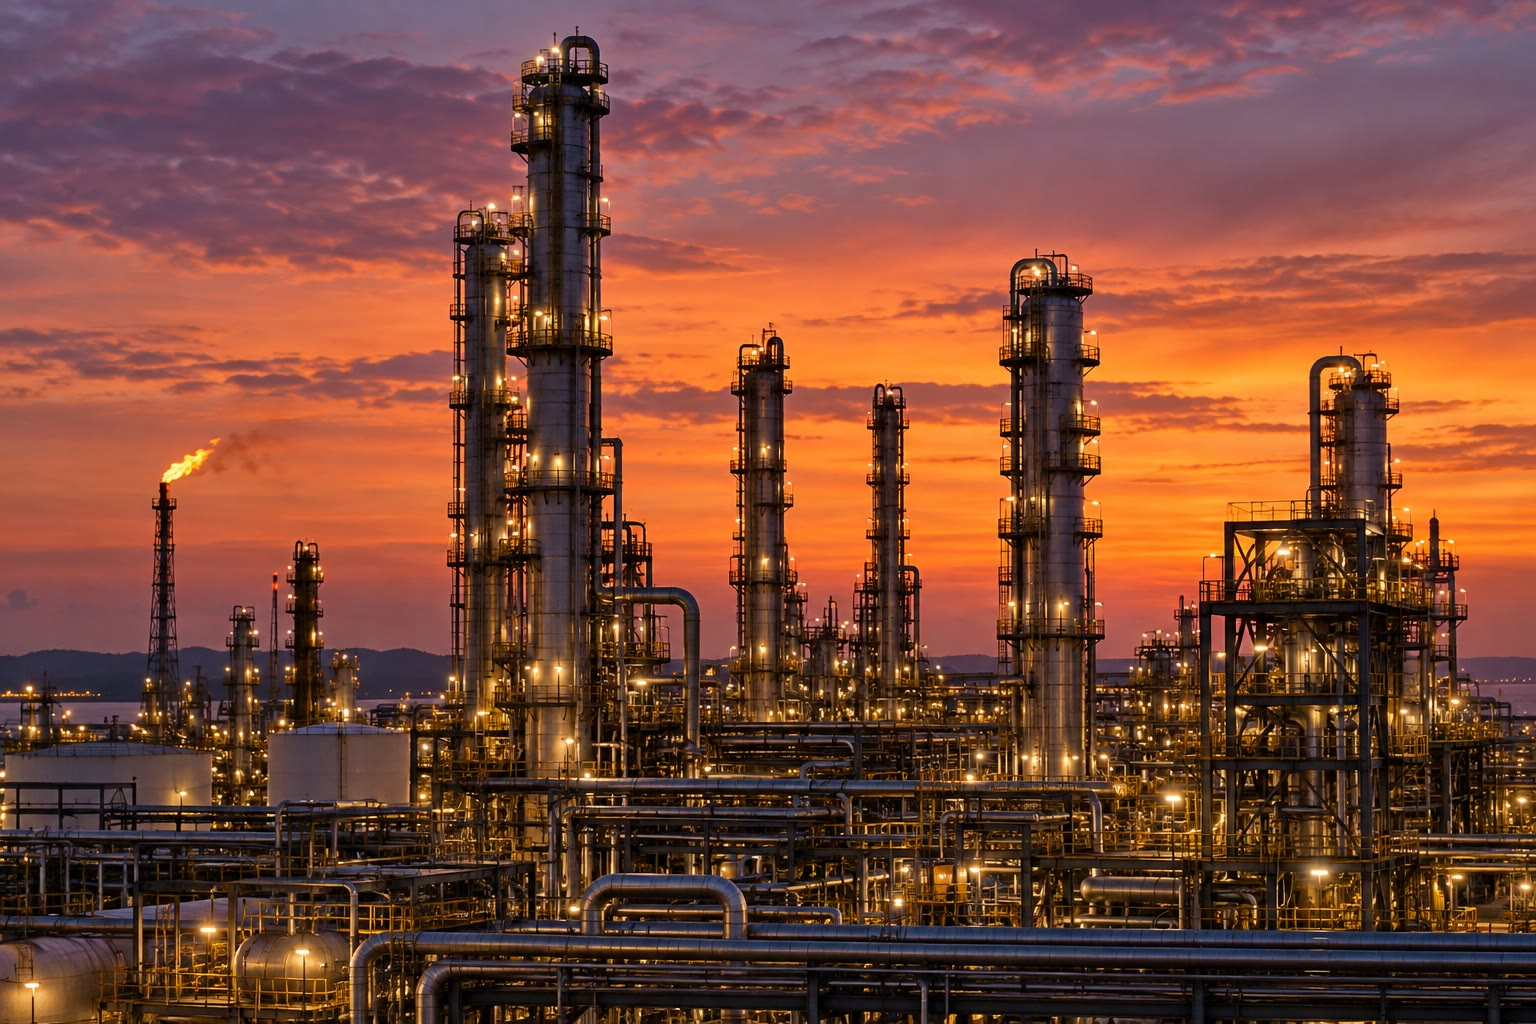
\includegraphics[width=0.52\linewidth]{images/book1/ai/g11-refinery-dusk.jpg}

{\small Les colonnes de \omterm{def:g10:chemical-species:distillation}{distillation} d'une raffinerie au crépuscule.}
\end{omfigure}

\begin{safety}{\ghs[0.66cm]{GHS02}\ghs[0.66cm]{GHS04}\ghs[0.66cm]{GHS07}\ghs[0.66cm]{GHS08}\ghs[0.66cm]{GHS09}}
% ledger: ghs:butane, ghs:pentane
Le butane est un gaz extrêmement inflammable, conservé sous pression. Le
pentane est un liquide très inflammable~; sa vapeur provoque la
somnolence, il peut endommager les poumons en cas d'ingestion et il est
toxique pour les organismes aquatiques. Aucune flamme près des \omterm{def:g11:organic-skeletons:alkane}{alcanes}
légers~; travailler sous une hotte.
\end{safety}

\section{Exercices}


\begin{exercise}[$\star$]\label{exo:g11:organic-skeletons:1}
Donner les \omterm{def:g11:organic-skeletons:formulas}{formules brutes} des \omterm{def:g7:atoms-and-molecules:molecule}{molécules} dessinées ci-dessous, et dire
si ce sont des \omterm{def:g11:organic-skeletons:isomer}{isomères}~:
\setchemfig{atom sep=1.6em}
\chemfig{-[:30]-[:-30]-[:30]-[:-30]-[:30]} \quad et \quad
\chemfig{-[:30](-[:90])-[:-30]-[:30]-[:-30]}.
\end{exercise}

\begin{exercise}[$\star$]\label{exo:g11:organic-skeletons:2}
Nommer~: \ce{CH3-CH2-CH3}~; \ce{CH3-CH2-CH2-CH2-CH2-CH3}~;
\chemfig{CH_3-CH(-[2]CH_3)-CH_2-CH_3}.
\end{exercise}

\begin{exercise}[$\star$]\label{exo:g11:organic-skeletons:3}
Écrire les \omterm{def:g11:organic-skeletons:formulas}{formules semi-développées} du propane et du 2-méthylpropane, et
la \omterm{def:g11:organic-skeletons:formulas}{formule développée} de l'éthane.
\end{exercise}

\begin{exercise}[$\star$]\label{exo:g11:organic-skeletons:4}
Compter les \omterm{def:g7:atoms-and-molecules:atom}{atomes} de carbone et d'hydrogène de chaque \omterm{def:g7:atoms-and-molecules:molecule}{molécule}~:
\setchemfig{atom sep=1.6em}
\chemfig{-[:30]-[:-30](-[:-90])-[:30]-[:-30]} \quad et \quad
\chemfig{*6(------)}.
\end{exercise}

\begin{exercise}[$\star$]\label{exo:g11:organic-skeletons:5}
Donner la \omterm{def:g11:organic-skeletons:formulas}{formule brute} de l'\omterm{def:g11:organic-skeletons:alkane}{alcane} à 8 \omterm{def:g7:atoms-and-molecules:atom}{atomes} de carbone, et le nombre
d'\omterm{def:g7:atoms-and-molecules:atom}{atomes} de carbone de l'\omterm{def:g11:organic-skeletons:alkane}{alcane} à 20 \omterm{def:g7:atoms-and-molecules:atom}{atomes} d'hydrogène.
\end{exercise}

\begin{exercise}[$\star\star$]\label{exo:g11:organic-skeletons:6}
Dessiner les \omterm{def:g11:organic-skeletons:formulas}{formules topologiques} du 3-méthylhexane, du
2,2-diméthylbutane et du 3-éthylpentane, et donner leurs \omterm{def:g11:organic-skeletons:formulas}{formules
brutes}.
\end{exercise}

\begin{exercise}[$\star\star$]\label{exo:g11:organic-skeletons:7}
Dessiner et nommer les trois \omterm{def:g11:organic-skeletons:isomer}{isomères} de \ce{C5H12}.
\end{exercise}

\begin{exercise}[$\star\star$]\label{exo:g11:organic-skeletons:8}
Ces noms sont faux. Dessiner chaque \omterm{def:g7:atoms-and-molecules:molecule}{molécule} et donner son nom
correct~: 2-éthylbutane~; 4-méthylpentane~; 1-méthylbutane.
\end{exercise}

\begin{exercise}[$\star\star$]\label{exo:g11:organic-skeletons:9}
À l'aide de la figure des \omterm{def:g11:organic-skeletons:isomer}{isomères} de \ce{C5H12}, les classer par
température d'ébullition et expliquer cet ordre.
\end{exercise}

\begin{exercise}[$\star\star$]\label{exo:g11:organic-skeletons:10}
Le cyclohexane a pour formule \ce{C6H12} et l'hexane \ce{C6H14}.
Expliquer les deux \omterm{def:g7:atoms-and-molecules:atom}{atomes} d'hydrogène manquants. Les deux composés
sont-ils \omterm{def:g11:organic-skeletons:isomer}{isomères}~? Le cyclohexane est-il un \omterm{def:g11:organic-skeletons:alkane}{alcane}~?
\end{exercise}

\begin{exercise}[$\star\star$]\label{exo:g11:organic-skeletons:11}
Parmi le propane, le butane, le 2-méthylpropane et le cyclobutane
(\ce{C4H8}, un cycle de quatre \omterm{def:g7:atoms-and-molecules:atom}{atomes} de carbone), lesquels sont \omterm{def:g11:organic-skeletons:isomer}{isomères}
les uns des autres~?
\end{exercise}

\begin{exercise}[$\star\star\star$]\label{exo:g11:organic-skeletons:12}
Dessiner et nommer les cinq \omterm{def:g11:organic-skeletons:isomer}{isomères} de \ce{C6H14}.
\end{exercise}

\begin{exercise}[$\star\star\star$]\label{exo:g11:organic-skeletons:13}
Représenter un \omterm{def:g11:organic-skeletons:alkane}{alcane} linéaire comme un long zigzag et un \omterm{def:g11:organic-skeletons:alkane}{alcane} très
ramifié comme une boule. À l'aide de cette image, expliquer pourquoi la
ramification abaisse la température d'ébullition des \omterm{def:g11:organic-skeletons:isomer}{isomères}.
\end{exercise}

\begin{exercise}[$\star\star\star$]\label{exo:g11:organic-skeletons:14}
Nommer l'\omterm{def:g11:organic-skeletons:alkane}{alcane}
\begin{center}
\chemfig{CH_3-CH(-[2]CH_3)-CH_2-C(-[2]CH_3)(-[6]CH_3)-CH_2-CH_3}
\end{center}
\end{exercise}

\begin{exercise}[$\star\star\star$]\label{exo:g11:organic-skeletons:15}
Le composé de référence pour l'essence, l'«~isooctane~», est le
2,2,4-triméthylpentane. Dessiner sa \omterm{def:g11:organic-skeletons:formulas}{formule topologique}, vérifier que
c'est un \omterm{def:g11:organic-skeletons:isomer}{isomère} de l'octane, et écrire sa \omterm{def:g11:organic-skeletons:formulas}{formule semi-développée}.
\end{exercise}

\section{Problème~: le gaz des briquets}

\begin{problem}[{Problème du week-end --- combien d'\omterm{def:g11:organic-skeletons:alkane}{alcanes} différents ont
pour formule \ce{C7H16}~?}]
\label{pb:g11:organic-skeletons:1}
% ledger: bp:C3H8, bp:C4H10, bp:isobutane
Un briquet contient du butane~; une cartouche de camping d'hiver contient
un \omterm{def:g6:pure-substances-and-mixtures:mixture}{mélange} plus riche en propane ou en 2-méthylpropane. Le butane bout
vers \qty{0}{\celsius}, le 2-méthylpropane à \qty{-11.7}{\celsius} et le
propane à \qty{-42}{\celsius}.

\medskip
\noindent\textbf{Partie I --- Deux gaz pour une formule.}
\begin{enumerate}
  \item Donner la \omterm{def:g11:organic-skeletons:formulas}{formule brute} du butane, et vérifier qu'elle correspond
        à la formule générale des \omterm{def:g11:organic-skeletons:alkane}{alcanes}.
  \item Dessiner sa \omterm{def:g11:organic-skeletons:formulas}{formule développée}.
  \item Écrire ses \omterm{def:g11:organic-skeletons:formulas}{formules semi-développée} et topologique.
  \item Représenter le 2-méthylpropane des trois mêmes façons. Pourquoi
        a-t-il la même \omterm{def:g11:organic-skeletons:formulas}{formule brute}~?
  \item Le butane et le 2-méthylpropane sont-ils \omterm{def:g11:organic-skeletons:isomer}{isomères}~? De quelle
        sorte~?
\end{enumerate}

\medskip
\noindent\textbf{Partie II --- Dans le froid.}
\begin{enumerate}[resume]
  \item Lesquels des trois gaz sont gazeux à \qty{20}{\celsius} sous la
        pression normale~?
  \item Un briquet ouvert est utilisé dehors à \qty{-5}{\celsius}.
        Pourquoi donne-t-il une mauvaise flamme~?
  \item Pourquoi les cartouches d'hiver sont-elles riches en propane ou
        en 2-méthylpropane~?
  \item Expliquer pourquoi le 2-méthylpropane bout plus bas que le
        butane.
  \item Pourquoi le propane n'a-t-il pas d'\omterm{def:g11:organic-skeletons:isomer}{isomère}~?
\end{enumerate}

\medskip
\noindent\textbf{Partie III --- Nommer et compter.}
\begin{enumerate}[resume]
  \item Nommer \chemfig{CH_3-CH(-[2]CH_3)-CH_2-CH_3}.
  \item Pourquoi le nom «~3-méthylbutane~» est-il faux pour la même
        \omterm{def:g7:atoms-and-molecules:molecule}{molécule}~?
  \item Combien d'\omterm{def:g11:organic-skeletons:alkane}{alcanes} \omterm{def:g11:organic-skeletons:isomer}{isomères} ont pour formules \ce{C4H10},
        \ce{C5H12} et \ce{C6H14}~?
\end{enumerate}

\medskip
\noindent\textbf{Partie IV --- Les \omterm{def:g11:organic-skeletons:isomer}{isomères} de \ce{C7H16}.}
\begin{enumerate}[resume]
  \item Dessiner l'\omterm{def:g11:organic-skeletons:isomer}{isomère} linéaire et le nommer.
  \item Dessiner et nommer les \omterm{def:g11:organic-skeletons:isomer}{isomères} dont la plus longue chaîne compte
        six \omterm{def:g7:atoms-and-molecules:atom}{atomes} de carbone. Pourquoi n'y a-t-il pas de
        «~4-méthylhexane~»~?
  \item Dessiner et nommer les \omterm{def:g11:organic-skeletons:isomer}{isomères} dont la plus longue chaîne compte
        cinq \omterm{def:g7:atoms-and-molecules:atom}{atomes} de carbone et deux groupes méthyle.
  \item Existe-t-il un \omterm{def:g11:organic-skeletons:isomer}{isomère} avec une chaîne de cinq carbones et un
        groupe éthyle~? Pourquoi le groupe éthyle ne peut-il se trouver
        que sur le carbone 3~?
  \item Dessiner et nommer l'\omterm{def:g11:organic-skeletons:isomer}{isomère} dont la plus longue chaîne compte
        quatre \omterm{def:g7:atoms-and-molecules:atom}{atomes} de carbone.
  \item Compter tous les \omterm{def:g11:organic-skeletons:isomer}{isomères} trouvés.
  \item Donner la réponse finale~: combien d'\omterm{def:g11:organic-skeletons:isomer}{isomères de constitution}
        l'heptane possède-t-il, lui-même compris~?
\end{enumerate}
\end{problem}
